\documentclass[letterpaper, 10 pt, conference]{ieeeconf}  % Comment this line out
                                                          % if you need a4paper
%\documentclass[a4paper, 10pt, conference]{ieeeconf}      % Use this line for a4
                                                          % paper

\IEEEoverridecommandlockouts                              % This command is only
                                                          % needed if you want to
                                                          % use the \thanks command
\overrideIEEEmargins
% See the \addtolength command later in the file to balance the column lengths
% on the last page of the document

\usepackage[pdftex]{graphicx}
\usepackage[font={footnotesize}]{caption,subfig}
% TODO remember we need to meet color compliance:
% http://its.papercept.net/conferences/support/general.php

\title{\LARGE \bf
Approximately Orchestrated Routing and Transportation Analyzer:\\
Large-scale Traffic Simulation for Autonomous Vehicles
}

\author{Dustin Carlino, Mike Depinet, Piyush Khandelwal, and Peter Stone\\
        Department of Computer Science\\
        The University of Texas at Austin\\
        Austin, TX 78712\\
        {\tt \small\{dcarlino,msd775,piyushk,pstone\}@cs.utexas.edu}}

\long\def\commentp#1{{\bf **Peter: #1**}}
\long\def\commentpk#1{{\bf **Piyush: #1**}}
\long\def\commentm#1{{\bf **Mike: #1**}}
\long\def\commentd#1{{\bf **Dustin: #1**}}
\long\def\commentc#1{{\bf **Chiu: #1**}}

% \long\def\commentp#1{}
% \long\def\commentpk#1{}
% \long\def\commentm#1{}
% \long\def\commentd#1{}
% \long\def\commentc#1{}

\begin{document}

\maketitle
\thispagestyle{empty}
\pagestyle{empty}

%%%%%%%%%%%%%%%%%%%%%%%%%%%%%%%%%%%%%%%%%%%%%%%%%%%%%%%%%%%%%%%%%%%%%%%%%%%%%%%%

\begin{abstract} 

Autonomous vehicles have seen great advancements in recent years, and such
vehicles are now closer than ever to being commercially available. The advent of
driverless cars provides opportunities for optimizing traffic in ways not
possible before. This paper introduces an open source multiagent microscopic
traffic simulator called AORTA, which stands for \textit{Approximately
Orchestrated Routing and Transportation Analyzer}, designed for optimizing
autonomous traffic at a city-wide scale. AORTA creates scale simulations of the
real world by generating maps using publicly available road data from
\textit{OpenStreetMap} (OSM). This allows simulations to be set up through
AORTA for a desired region anywhere in the world in a matter of minutes. AORTA
allows for traffic optimization by creating intelligent behaviors for
individual driver agents and intersection policies to be followed by these
agents. These behaviors and policies define how agents interact with one
another, control when they cross intersections, and route agents to their
destination. This paper demonstrates a simple application using AORTA through
an experiment testing intersection policies at a city-wide scale.

\end{abstract}

%%%%%%%%%%%%%%%%%%%%%%%%%%%%%%%%%%%%%%%%%%%%%%%%%%%%%%%%%%%%%%%%%%%%%%%%%%%%%%%%

\section{INTRODUCTION}
\label{sec:introduction}

Autonomous vehicle technology has made tremendous progress in the last decade.
In 2007, six of the competing teams completed the 96km course set for the DARPA
Urban Challenge \cite{spectrumUrbanChallenge2007}. They did so while
obeying the traffic laws followed by human drivers, navigating along with other
moving vehicles, and following correct intersection precedence order. Since
then, Google's driverless cars have clocked more than 250,000km on public roads
in urban California, USA \cite{tedThrun2011}. In 2010, researchers from the
University of Parma successfully completed an autonomous
\textit{intercontinental} run from Parma, Italy to Shanghai, China
\cite{cnnVislab2010}. The successful completion of all these milestones
suggests that autonomous cars are here to stay, and are ever closer to becoming
commercially available. With the arrival of autonomous cars, it also becomes
possible to optimize traffic in ways not possible for human drivers. 

% The arrival of driverless cars presents several challenges that need to be
% addressed in the near term. Road infrastructure changes could provide important
% improvements to traffic involving autonomous vehicles. A number of legal and
% safety concerns need to be addressed in the context of driverless cars. Human
% drivers need new methodologies to interact with autonomous drivers on public roads.
% This work aims to solve some of these problems by providing a sandbox in which such
% methodologies can be found and tested for safety and efficiency before being
% deployed in the real world.  In this manner, the present work aids in the effort to find
% intermediate stages between entirely human and entirely autonomous traffic.

\begin{figure}[t]
  \centering 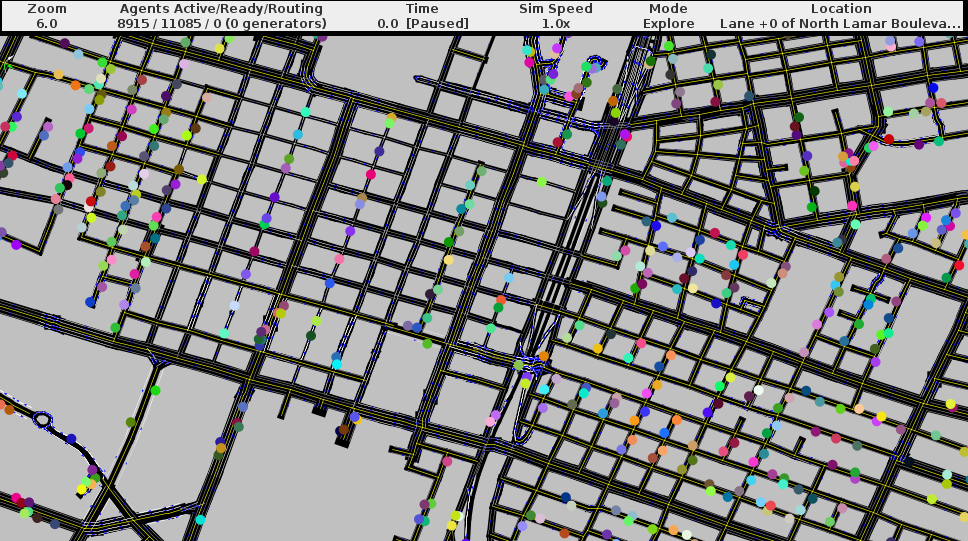
\includegraphics[width=0.9\linewidth]{downtown_atx.png}
  \caption{Visualizing autonomous agents in downtown Austin, Texas, with AORTA's UI}
  \label{fig:ui_screenshot}
  \vspace{-20pt}
\end{figure}

% TODO reference the screenshot

This paper introduces an open source multigent microscopic traffic simulator
called AORTA, which stands for \textit{Approximately Orchestrated Routing and
Transportation Analyzer}. AORTA is a platform designed for testing autonomous
vehicle behaviors and intersection policies. Autonomous vehicles, termed agents,
use behaviors to interact with one another, follow intersection policies, and
decide on both long term and short term actions. Intersection policies designate
when it is safe for an agent to cross an intersection.  AORTA's goal is to allow
for the definition of new agent behaviors and intersection policies to optimize
autonomous traffic. Additionally, by assigning human-like behaviors such as the
``car following model'' \cite{brackstone1999car} to agents and
traffic-signal-like policies to intersections, AORTA could potentially simulate
human traffic.

Like any other microscopic traffic simulator, AORTA needs maps to run
simulations. One of AORTA's key features is that it generates maps using real
road data available from OpenStreetMap (OSM) \cite{osm}, a moderated,
user-editable interface for world maps. A map for any desired city in the world
can be downloaded, which is then parsed by AORTA to set up a scale simulation
of the real world in a few minutes. AORTA is available open-source and is
easily extensible\footnote{Code available at
\texttt{http://code.google.com/p/road-rage}}, making it easier for users to
test out a number of agent behaviors and intersection policies in a short
time span.

This paper explores the state-of-the-art in traffic simulators in section
\ref{sec:related_work}, followed by a description of AORTA's architecture in
section \ref{sec:arch}.  Use of OSM data in AORTA is explained in section
\ref{sec:map}, along with a description of the simulator in section
\ref{sec:simulation}. Section \ref{sec:results} demonstrates an application
built on top of AORTA and presents a simple experiment evaluating different
intersection policies in a large scale scenario. The paper then concludes with a
discussion on future work.

%%%%%%%%%%%%%%%%%%%%%%%%%%%%%%%%%%%%%%%%%%%%%%%%%%%%%%%%%%%%%%%%%%%%%%%%%%%%%%%%

\section{RELATED WORK}
\label{sec:related_work}

Computational processing power has made excellent advancements in the last two
decades. Parallel computing and the use of GPUs have enabled microscopic models
of traffic simulation to generate results at a meaningful scale (city-wide or
greater) \cite{nagel1994microscopic,shen2011agent}. As a result, a number of
multiagent micro-simulators have been introduced in the past decade. We review
relevant simulators and other related work in this section.

OSM data has been used by traffic simulators in the past. MATSim is one such
multiagent simulator that focuses on performing large-scale simulations in a
relatively small amount of time \cite{balmer2009matsim}. Traffic demand is
supplied to MATSim in the form of \textit{plans} that an individual may intend
to follow in a given day. MATSim aims to improve these plans by attempting to
minimize the total amount of time by which individuals are late to their
destinations. This goal is somewhat different from that of AORTA, where the
routes (demand) supplied by individuals is taken as is. Instead, AORTA focuses
on vehicle behaviors and intersection policies to improve the execution of
routes.

Another popular open source traffic simulator that can use OSM data is SUMO
\cite{SUMO2011}, which shares many similar goals with AORTA. SUMO has been used to
study the effect of automated transportation systems, route planning of
individual vehicles, as well as dynamically adapting traffic signal policies to
increase traffic efficiency. While SUMO has a flexible system for managing
traditional traffic signals, AORTA's general intersection policies are designed
with autonomous vehicles in mind. These policies can use traditional schemes
such as traffic signals or stop-sign based precedence, or more efficient methods
designed specifically for autonomous vehicles \cite{JAIR08-dresner}. In
addition, AORTA's core implementation, written in Scala \cite{scala}, differs
from that of SUMO, written in C++, in that it uses a higher-level language.

Efforts have been made to optimize traffic flow in the context of autonomous
vehicles. AIM \cite{JAIR08-dresner} is one such approach that aims to optimize
traffic flow of autonomous vehicles at a given intersection. The AIM approach
has been applied to a regular grid of four intersections
\cite{IROS11-hausknecht}, while AORTA has the potential to apply some of the
same research at a city-wide scale to real-world road networks.

% Simulators have also focused on autonomous vehicles with sensors and actuators
% \cite{figueiredo2009approach}. These simulators are used to ensure that
% autonomous vehicles are behaving correctly while interacting with other
% vehicles and infrastructure, given their configuration of sensors and
% actuators. On the other hand, AORTA assumes that autonomous vehicles have
% reasonable sensory input and mechanical output, and instead focuses on
% interactions between an agent and its surrounding agents and intersections.

Autonomous agents have also been used in the past to model human traffic. For
instance, one approach models human merging and lane changing behavior through
the use of autonomous agents interacting with one another
\cite{hidas2002modelling}. Another approach attempted to improve traffic
congestion for human drivers by using a network of autonomous intersections.
These intersections have the ability to interact with one another and execute a
dynamic traffic signal policy minimizing overall wait time
\cite{manikonda2001autonomous}.

%%%%%%%%%%%%%%%%%%%%%%%%%%%%%%%%%%%%%%%%%%%%%%%%%%%%%%%%%%%%%%%%%%%%%%%%%%%%%%%%

\section{ARCHITECTURE}
\label{sec:arch}

% Diagram made with gliffy.com. architecture.gxml should enable editing.
\begin{figure}
  \centering 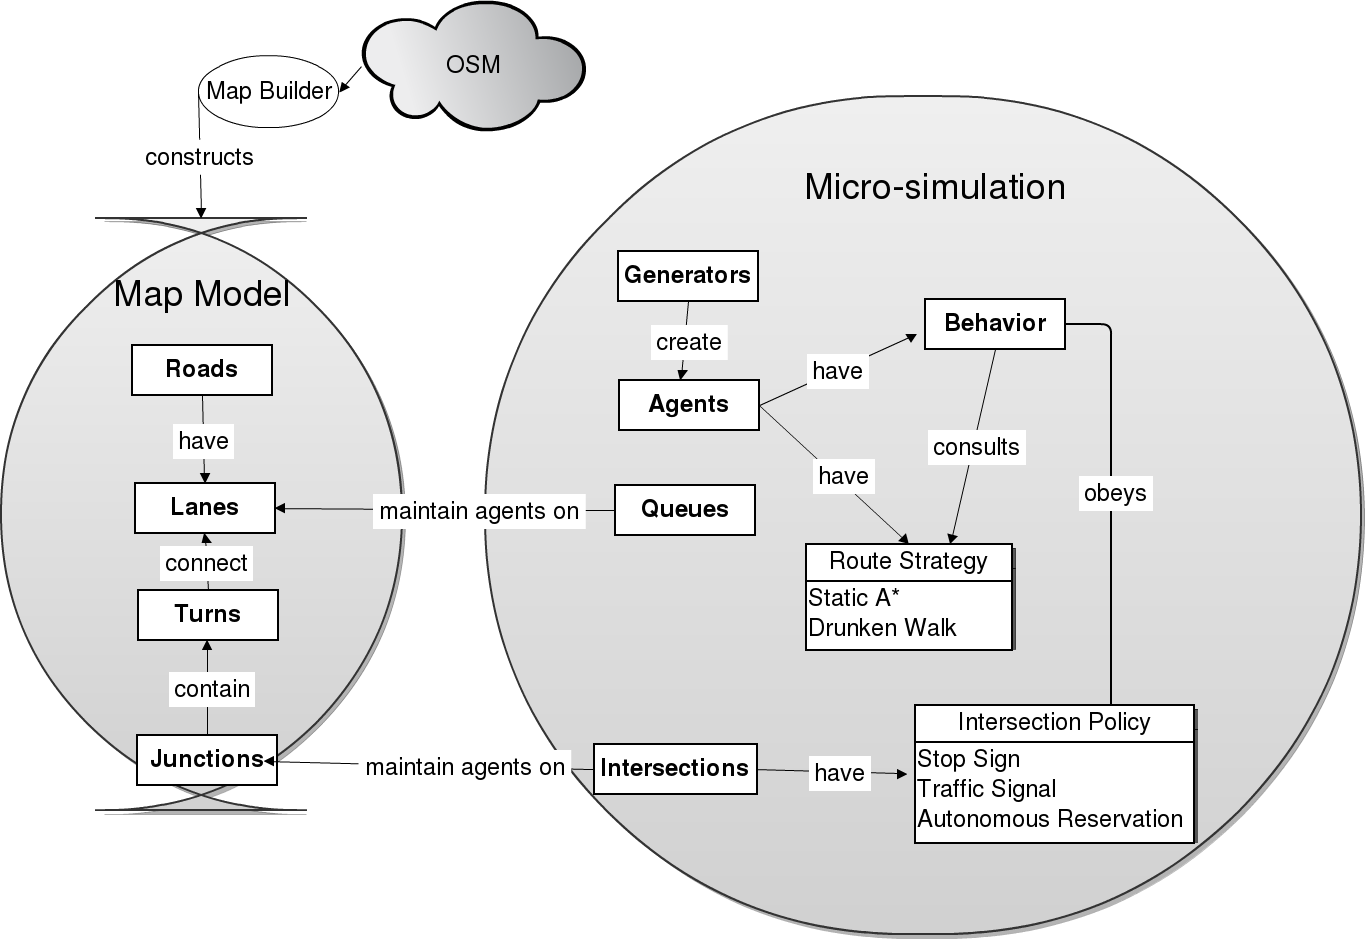
\includegraphics[scale=0.3]{architecture.png}
  \caption{A summary of AORTA's components.}
  \label{fig:arch}
  \vspace{-15pt}
\end{figure}

AORTA is divided into three modular components: the map model, micro-simulation
engine, and user interface (UI). The map model transforms OSM maps into AORTA
graphs, then answers pathfinding and geometry queries. The simulation engine
adds a notion of agents, vehicle dynamics, and collisions. Finally, the UI
interactively renders the map and agents. A headless mode also exists to run
experiments without the overhead of visualization. The interaction between
modules is visualized in figure \ref{fig:arch}.

AORTA's implementation uses Scala, a language implemented on the Java Virtual
Machine \cite{scala}. Scala provides the advantage of functional programming
constructs while still permitting imperative style.  Extensions and clients
built on top of AORTA can be written in either Java or Scala. The software is
open-source and easily extensible. For instance, the stop sign sign policy used
in experiments described in section \ref{sec:results} is implemented in just 70
lines of code. 

Sections \ref{sec:map} and \ref{sec:simulation} describe map construction from
OSM data and the simulation engine used in the AORTA framework respectively.

%%%%%%%%%%%%%%%%%%%%%%%%%%%%%%%%%%%%%%%%%%%%%%%%%%%%%%%%%%%%%%%%%%%%%%%%%%%%%%%%

\section{MAP CONSTRUCTION FROM OSM}
\label{sec:map}

One of the key features of AORTA is the simulation of traffic on existing road
network data from OpenStreetMap \cite{osm}. The data from OSM is not directly
suitable for running a simulation and is pre-processed through a \emph{map
builder} utility. Section \ref{sec:mapmodel} describes the map model generated
by the builder, section \ref{sec:mapconstruction} describes the process of
refining OSM data, and section \ref{sec:osmlimits} describes limitations with
this process.

\subsection{Map Model}
\label{sec:mapmodel}

A map is represented as a directed graph with \emph{lanes} as edges and
\emph{turns} as vertices. A \emph{road} groups a set of lanes together, one set
for each direction of travel. \emph{Intersections} map the possible turns from
incoming to outgoing lanes. Since both lanes and turns support traffic, they
are both called \emph{traversables}, meaning agents may exist on them.

The map also has a geometric interpretation, used for visualization and
measuring physical distances. A road contains a sequence of points, defining
the center line that divides the road into two directions of travel. AORTA
interprets these points as straight lines and projects parallel lanes out using
a fixed width. Turns are modeled with a single straight line connecting the end
of one lane to the start of another.

\subsection{Map Construction Passes}
\label{sec:mapconstruction}

The builder works incrementally while parsing OSM graphs into the map model,
with each pass feeding the next. The map model is then stored in an XML format.
\begin{enumerate}
  \item OSM encodes many paths besides drivable roads, so the builder first filters
        these out. Next, the builder marks OSM nodes common to multiple roads, since
        they implicitly indicate intersections. Overpasses do not share nodes
        with the roads they cross \cite{osmOverpass}.
  \item OSM \emph{ways} (sequences of nodes) include many
        intersections, so the builder next splits ways into undirected
        segments of roads between exactly two intersections.
  \item The builder multiplies undirected roads into directed lanes in each
        direction (unless the road is marked one-way). The builder guesses the
        number of lanes based on OSM's ``road type'' tag or an explicit number of
        lanes, when that data is available.
  \item The builder constructs turns between incoming and outgoing lanes at each
        intersection. The angle between the two lanes determines whether the turn is
        a left, right, straight, or U-turn. When several lanes all cross into fewer
        lanes, the builder forces merging at the rightmost lanes. 
  \item Because turns are heuristically placed, the graph is often disconnected.
        In order to ensure that an agent will be able to reach any point in the map,
        the builder removes all but the largest strongly connected component of the
        directed graph. Disconnected lanes are spliced out of larger roads, leaving
        geometric gaps, but correctly ensuring connectivity.
\end{enumerate}

\subsection{Limitations with OSM}
\label{sec:osmlimits}

AORTA's map construction process, although flexible, cannot completely account
for incompleteness in OSM data. Road type annotations imprecisely imply the
number of lanes and typical speed limits. Heuristically enumerating the turns at
each intersection often misses common features like right turn-only lanes and
shared center left turn lanes. There are many circumstances where AORTA
simulates one intersection as several in close proximity because roads do not
geometrically line up, but functionally they do. If OSM encoded this data, the
the realism of the simulation would improve. Other simulators have identified
similar issues before \cite{Krajzewicz_Hertkorn_Ringel_Wagner_2005}.

%%%%%%%%%%%%%%%%%%%%%%%%%%%%%%%%%%%%%%%%%%%%%%%%%%%%%%%%%%%%%%%%%%%%%%%%%%%%%%%%

\section{SIMULATION}
\label{sec:simulation}

This section describes AORTA's agent model and the simulator's mechanisms for
creating agents, verifying safety, and allowing agents and intersections to
control themselves. Comments on current limitations and how to extend the
simulator follow.

\subsection{Simulation Dynamics} 

AORTA uses microscopic simulation, modeling individual drivers as point agents
with a simple acceleration-based dynamics model. Time is modeled discretely,
and an agent accelerates at a fixed rate for the duration of a ``step'' to
achieve a new position and velocity. Space is continuous, meaning agents occupy
a moving interval of a lane, rather than one fixed tile of the road. Each time
step lasts for the same fixed duration, and the simulation does the following
for each time step:

\begin{enumerate}
  \item Introduces new agents into the map
  \item Updates the position and velocity of agents based on their choice of
        acceleration in the previous step
  \item Checks for collisions
  \item Allows each agent's behavior to choose an action for the next step
\end{enumerate}

\subsection{Spawning new agents}

To introduce new agents into the simulation in real-time, users can create
\emph{generators} programatically or using the UI. The generator produces the
desired amount of traffic by initializing agents from random locations inside a
\textit{start} polygon to random destinations within a \textit{goal} polygon.
Users can draw these polygons by mouse in the UI, allowing specific traffic
patterns like rush-hour scenarios to be easily simulated. A generator polygon
may also cover the entire map, uniformly distributing traffic everywhere.

Every step, a generator creates some number of new agents. The generator either
immediately performs any timely computation required by the agent's route
policy, such as pathfinding, or delegates it to a pool of worker threads to
process in the background.  Once an agent's route is ready, the agent waits
alongside its starting lane (as if it is in a driveway or parking lot). When the
lane has no agents that could potentially crash into the new vehicle, the new
agent enters the system.

\subsection{Collision checking}

All traversables (lanes and turns) maintain an ordered queue of occupying
agents. A collision is detected when two agents reverse order after a time step
has completed.

Intersections check for collisions by verifying no two agents are simultaneously
performing conflicting turns. AORTA has a low-granularity model of turn
conflict. If two vehicles at any point along two different turns could ever come
into contact, then the turns are always in conflict, no matter where the agents
actually are along that turn. This is visualized in figure \ref{fig:conflicts}.
Further work is required before higher granularity can be introduced through
space-time tiling intersections \cite{JAIR08-dresner}, due to some of the
complex intersection geometries inferred from OSM. An example of such a complex
intersection is shown in figure \ref{fig:crazyIntersection}.

% When a collision occurs, the simulator throws warnings and halts, since this
% indicates a bug in some policy. A future alternative could be to mark the region
% as impassable and re-route other traffic away from the accident.

\begin{figure}[h]
  \centering
  \subfloat[An agent cannot turn left while agents on the perpendicular road
  cross]{
    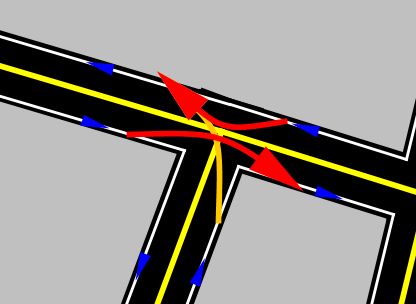
\includegraphics[width=0.42\columnwidth]{turn_conflicts.png}
    \label{fig:conflicts}
  }
  ~ % horizontal spacing, mostly for the sake of the captions
  \subfloat[A difficult intersection to tile in New Orleans, Louisiana. Note
  there are no overpasses pictured.]{
    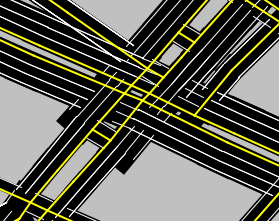
\includegraphics[width=0.4\columnwidth]{crazy_intersection.png}
    \label{fig:crazyIntersection}
  }
  \caption{Examples of AORTA's modeling of intersections and turns}
  \vspace{-15pt}
\end{figure}

\subsection{Agent Behaviors}

Each agent has a \emph{behavior} governing it, responsible for obeying
intersection policies and avoiding collisions. Before each step, the behavior
chooses one of two actions for the agent to perform: disappearing from the map
(when the agent is at rest and is done with its route) or accelerating at some
rate. Behaviors query current and upcoming lanes and intersections to find
other nearby agents and determine all constraints that must be satisfied for a
safe choice. The behavior also picks turns once an agent reaches the end of a
lane by consulting a route strategy that finds a path to the destination.

\subsection{Intersection Policies}
\label{sec:policies}

A behavior interacts with an intersection policy by sending it the agent's
desired turn, the agent's speed, the current distance from the start of the
intersection, and the length of time the agent has been idling at rest. The
policy replies by ordering the agent to \textit{stop} or \textit{proceed}. The behavior
will continue to statelessly poll the policy every step until the agent begins
the turn. The policy may approve an agent for entry one step and deny it the
next, as long as the agent could safely brake without danger of entering the
intersection. The policy is free to allow concurrent turns in any arrangement by
different agents as long as no two simultaneous turns conflict.

\subsection{Current Limitations}

Currently agents cannot change lanes. This causes a second issue: gridlock.
Each agent maintains a safe following distance from the next. If a lane is
filled, then an agent may be forced to stop in an intersection mid-turn and
block other traffic. The default behavior prevents this by refusing to start a
turn before the lookahead engine guarantees no agent will trigger a premature
stop.

However, with very high volumes of traffic, it is possible for waiting agents to
accumulate and fill lanes to their capacity. When this happens in a circular
manner so that the agent at the front of each lane is waiting to perform a turn
into another full lane with a similar agent at the front, gridlock
\cite{AAAI11-au} occurs: no agent in the system will make progress unless an
agent at the front decides to pick a different turn. AORTA has the ability to
find such cycles.

\begin{figure}[h]
  \centering 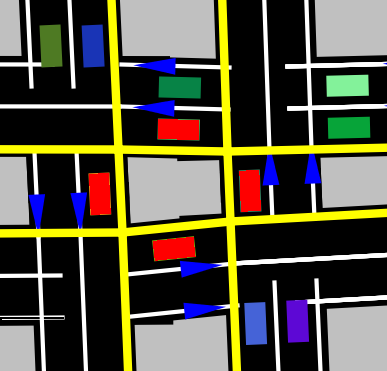
\includegraphics[scale=0.25]{gridlock.png}
  \caption{Each of the red agents wants to turn left, so none of them can.}
  \label{fig:gridlock}
  \vspace{-10pt}
\end{figure}

In many observed cases, the gridlock is caused by AORTA's present lack of
lane-changing support: agents loop around intersections such as those pictured
in figure \ref{fig:gridlock} in order to enter a lane adjacent to their original
lane.  Since these routes are still legal, it is desirable to prevent or mend
this problem without forcing different routes. However, choosing alternative
moves (by changing lanes or rerouting) is an important constituent of a
sufficient condition for the liveness of a road network \cite{AAAI11-au}.

\subsection{Extending AORTA}
\label{sec:config}

There are three main configurable components of the simulation, each with at
least one existing implementation: agent behaviors, routing strategies, and
intersection policies.

Currently, all agents use a primary behavior that is a generalized, baseline
behavior that guarantees not to collide with another agent or enter an
intersection at the wrong time. Since it picks the highest safe choice of
acceleration at each step, it could easily be extended to mimic human drivers by
traveling at some random lesser acceleration or to optimize fuel efficiency
by tuning movement.

Intersection policies are one of the most interesting aspects of the simulation
to tweak, especially in light of autonomous vehicles. Current policies include
traditional stop signs, traffic signals, and an AIM-inspired autonomous
reservation policy \cite{JAIR08-dresner}. The traffic signals are further
extensible by assigning groups of non-conflicting turns at each intersection
with some duration and offset. Future policies could include signals that adapt
timings and refinements to the autonomous reservation policy.

To pick turns, agent behaviors consult a route strategy. Two simple
implementations exist already: a static route using A* \cite{astar} and a
drunken walk that probabilistically moves towards the destination. Users can
experiment with dynamic replanning or hierarchical planning
\cite{Botea04nearoptimal} without modifying any code other than creating a new
route implementation. Route policies could also interact with a single central
manager to gain some sort of global insight or with autonomous intersections to
avoid congestion.

%%%%%%%%%%%%%%%%%%%%%%%%%%%%%%%%%%%%%%%%%%%%%%%%%%%%%%%%%%%%%%%%%%%%%%%%%%%%%%%%

\section{EXPERIMENTAL RESULTS}
\label{sec:results}

\begin{figure*}[t]
  \centering
  \subfloat[Average delay in Austin]{
    \label{fig:avg_lag_atx}
    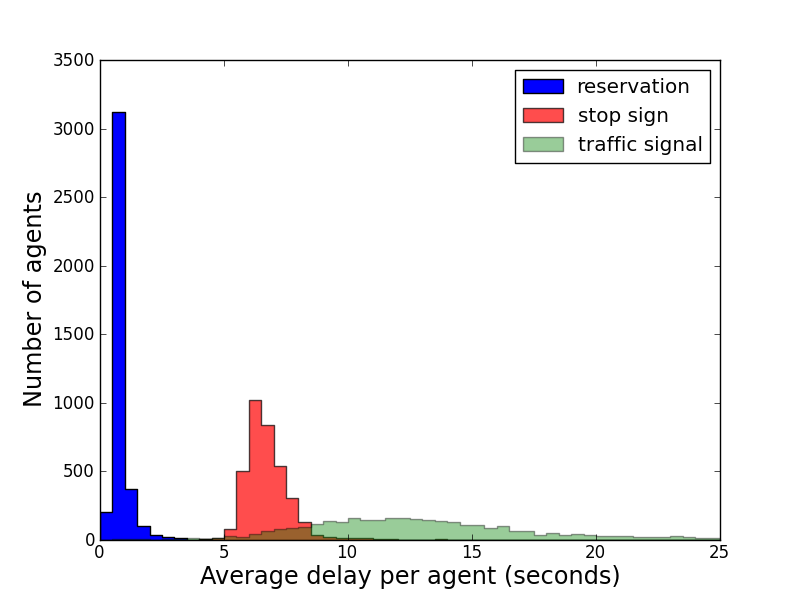
\includegraphics[width=0.4\textwidth]{avg_lag_agent_atx.png}
  }\,
  \subfloat[Average delay in Houston]{
    \label{fig:avg_lag_houston}
    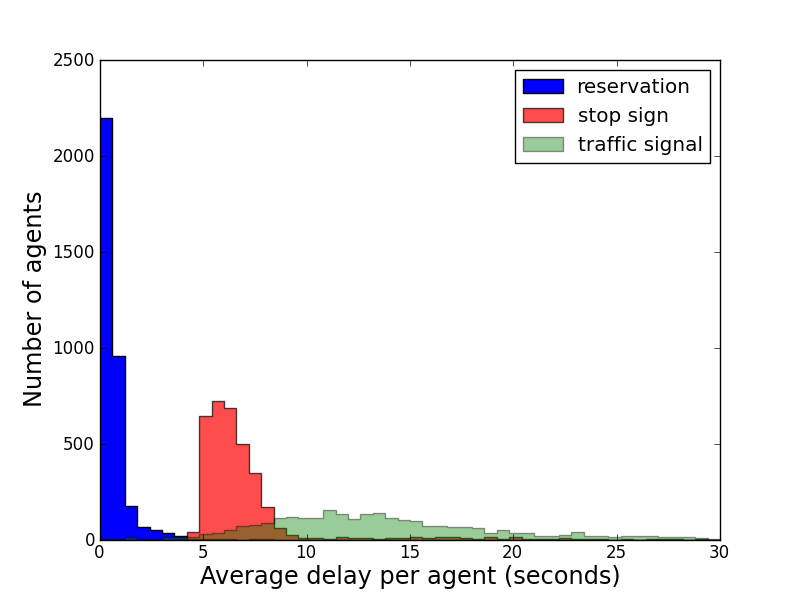
\includegraphics[width=0.4\textwidth]{avg_lag_agent_houston.png}
  }\\
  \subfloat[Number of agents driving in Austin]{
    \label{fig:agent_cnt_atx}
    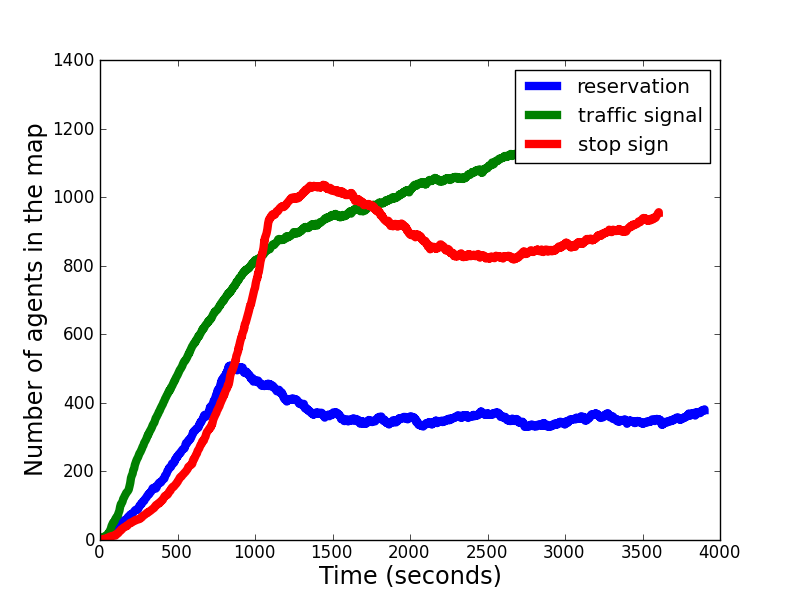
\includegraphics[width=0.4\textwidth]{agent_cnt_atx.png}
  }\,
  \subfloat[Number of agents driving in Houston]{
    \label{fig:agent_cnt_houston}
    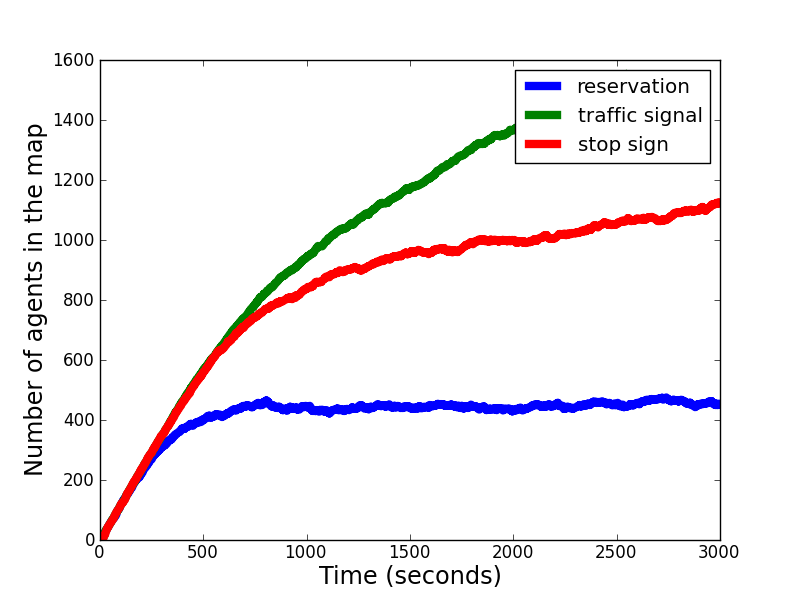
\includegraphics[width=0.4\textwidth]{agent_cnt_houston.png}
  }
  \caption{Autonomous reservations outperform stop signs and traffic signals in
           these experiments.}
  \label{fig:results}
  \vspace{-15pt}
\end{figure*}

This section presents a simple experiment showing how different policies affect
the throughput of intersections. In this experiment, every intersection in the
map uses either a stop sign, traffic signal, or autonomous reservation policy.
The results demonstrate that policies affect total system performance and that
AORTA is a useful tool for evaluating this relation.

\subsection{Experimental Setup}

The experiment simulates one hour of traffic in two cities: a
9$\times$11km$^{2}$ slice of downtown Austin, Texas\footnote{bounded by the
Mopac, Springdale Road, Oltorf Street and Koenig Lane}, and a
15$\times$13km$^{2}$ slice of downtown Houston, Texas\footnote{bounded by Ella
Boulevard, Eastex Freeway, West Alabama Street and Crosstimbers Street}.  The
step duration is fixed at 0.1 seconds. While the intersection policies vary,
the agents spawned and their routes remain the same.  A generator creates one
new agent every 1 simulation second, with a uniformly random starting position
and goal.

These experiments are deterministically reproducible. A seed for the
pseudo-random number generator, the input graph, and the generators'
configuration fully determine the outcome of any simulation \footnote{This
determinism may break down when generators use worker threads while the
simulation is running, since tasks may finish and agents may enter the road at
different times}. After setting up a scenario in the UI, users can save this
configuration for re-simulation.

The speed of simulation depends on the step duration $dt$, the map size, and the
number of agents. A measure independent of these factors is the number of agent
steps per second. On a 2.4 GHz machine, this can be observed to average at
about 150,000, a number comparable to existing simulators \cite{SUMOthesis}.
When the time step is 0.1 seconds, this means 15,000 agents can be comfortably
simulated in real-time. Further optimizations are planned.

\subsection{Intersection Policies Evaluated}

Stop signs accept agents first-come, first-served, refusing agents until they
have idled at rest for 1 second. This delay approximates human reaction time.

The traffic signal policy requires timings and groups of simultaneous turns for
each intersection. The heuristic currently assigning these arbitrarily picks one
major road, schedules turns from that road to others, then repeats the process
from all reachable roads using a breadth-first search. By estimating how long
performing one turn and traveling along the next lane takes, the timing of the
next intersection can be scheduled so that agents from the first road continue
traveling without stopping for several consecutive intersections. This heuristic
is far from optimal, meaning the performance of traffic signals described below
could be improved, perhaps by incorporating packages such as SYNCHRO
\cite{synchro}.

The last policy tested is an autonomous reservation policy inspired by AIM
\cite{JAIR08-dresner}. Because agents explicitly communicate with intersections
to schedule their turn, this policy is only suitable for autonomous drivers.
This policy groups agents with compatible turns together, allowing new agents to
join existing groups. To prevent one heavy direction of traffic from hogging the
intersection indefinitely, a timeout preemptively cycles through reservations.

\subsection{Results}

If an agent travels along a lane at the speed limit and does not slow down to
wait at an intersection, then it traverses the lane in an optimal amount of
time. If the intersection orders it to stop or if other agents in the same lane
have slowed down by the intersection's orders, then the intersection has caused
some delay. This delay can be used as one measure of intersection performance.
Figures \ref{fig:avg_lag_atx} and \ref{fig:avg_lag_houston} graph the average of
this delay per agent. Similar trends are observed in both cities: an average of
less than 1 second of delay at autonomous reservation intersections, 7 (Austin)
or 8 (Houston) seconds at stop signs, and 16 (Austin) or 17 (Houston) seconds at
traffic signals using the heuristic described above.  These results will vary
with different traffic levels and policy configurations, so the important
demonstration is that AORTA can be used as a framework for evaluating these
policies.

The number of agents driving at some time changes because the continuous
generator introduces a new agent every second. This count reaches a steady state
when the generator introduces an agent at the same rate as older agents finish
their route. Figure \ref{fig:agent_cnt_atx} reveals that autonomous reservations
let agents reach their destination twice as quickly as the competition in
Austin, with a steady-state of about 400 agents. There, the count for traffic
signals continues to increase because gridlock occurred in one segment of the
map, causing agents to not finish their route. Figure
\ref{fig:agent_cnt_houston} reveals a similar trend in Houston, except that
gridlock occurred both during the trial with traffic signals and stop signs.
Unexpected starvation was also observed: although the signals cycle through
turns regularly, agents cannot proceed when the previous cycle caused a
destination lane to fill and become blocked.

Repeating this or other experiments in more locations only requires those
locations to be exported from the OSM website. Editing the intersection policies
is similarly convenient, as users can ignore most of AORTA's code-base and just
change the logic described in section \ref{sec:policies}.  For reference, the
most complex intersection policy, traffic signals with the flooding heuristic
for timing assignment, is only 400 lines of code in Scala.

%%%%%%%%%%%%%%%%%%%%%%%%%%%%%%%%%%%%%%%%%%%%%%%%%%%%%%%%%%%%%%%%%%%%%%%%%%%%%%%%

\section{CONCLUSION}
\label{sec:conclusion}

This paper has presented AORTA, a new city-scale traffic simulation framework
that focuses on configurability. In conjunction with Open Street Maps, AORTA
allows users to repeat an experiment in different places with minimal effort.
Future work will exploit the flexible infrastructure of interactions between
agent behaviors and intersections by exploring dynamic replanning and adaptable
signal timings. On top of these structures, applications could experiment with
ideas such dynamic contra-flow \cite{ITSC11-hausknecht}.  There will also be an
effort to improve AORTA as a framework by including a lane-changing model,
preventing gridlock, and supporting more agents through parallel computing.

% \addtolength{\textheight}{-12cm}  % This command serves to balance the column lengths
%                                   % on the last page of the document manually. It shortens
%                                   % the textheight of the last page by a suitable amount.
%                                   % This command does not take effect until the next page
%                                   % so it should come on the page before the last. Make
%                                   % sure that you do not shorten the textheight too much.

%%%%%%%%%%%%%%%%%%%%%%%%%%%%%%%%%%%%%%%%%%%%%%%%%%%%%%%%%%%%%%%%%%%%%%%%%%%%%%%%
\section*{ACKNOWLEDGMENTS}

This work has taken place in the Learning Agents Research Group (LARG) at the
Artificial Intelligence Laboratory, The University of Texas at Austin. LARG
research is supported in part by grants from the National Science Foundation
(IIS-0917122), ONR (N00014-09-1-0658), and the Federal Highway Administration
(DTFH61-07-H-00030). 

The authors would like to thank Dr. Michael Quinlan for his support during the
seminal stages of AORTA and all OpenStreetMap contributors for collecting the
map data used in this work. Efforts by the Freshman Research Initiative,
College of Natural Sciences, UT Austin have allowed for the development of this
research.

%%%%%%%%%%%%%%%%%%%%%%%%%%%%%%%%%%%%%%%%%%%%%%%%%%%%%%%%%%%%%%%%%%%%%%%%%%%%%%%%

% They're sorted by order of citation, not alphabetically. IEEEtran.bst confirms
% this is the correct "numerical citation style."
\bibliographystyle{IEEEtran}
\bibliography{root}

\end{document}
